\section{Introduction}
\label{sec:intro}

%% Soft robots can do cool things because they are compliant, but are difficult to model and control for the same reason
Soft robots, or robots that incorporate non-rigid materials into their morphology to facilitate compliant interactions with the external world, are being developed for purposes such as manipulating delicate objects, adapting to unstructured environments, and enabling safe interactions with coexisting humans \cite{rus2015design}. \David{Yes, more references}
While such robots demonstrate physical capabilities beyond those of traditional rigid-bodied robots, their dynamic behavior is not well-understood \cite{george2018control}.
The infinite degrees of freedom and hysteretic \David{I haven't read further yet, but will your approach be able to handle hysteresis?} behavior of soft materials make it difficult to construct accurate physics-based models of soft robots without making significant simplifying assumptions such as constant curvature \cite{rus2015design}, quasi-static \cite{george2018control}, or simplified geometry \cite{bruder2017model, sedal2017constitutive, bishop2012parallel} \Ram{you are only referencing a handful of papers despite having an infinite amount of space for references. This is dangerous especially since our competitors are going to review this paper and will expect to be cited..}.
These models 
% \hl{suffer from the same shortcoming as linearizations of nonlinear models in that they}
only describe behavior well in the subset of robot configurations where all assumptions hold, hence they are limited in applicability \Ram{can you describe with a more concrete example what you mean?}.
\David{Talk to Audrey, she will no have a good perspective about why it is hard to model soft robots.  I think other issues not mentioned here are computational cost, identification of material properties, influence of manufacturing tolerances,...}
% white-box model based on first principles, e.g. a model for a physical process from the Newton equations, but in many cases such models will be overly complex and possibly even impossible to obtain in reasonable time due to the complex nature of many systems and processes

%% Lack of good models poses a problem for control
This lack of globally valid models poses a problem for control.
When a good enough model \Ram{what is good enough?}  is available, a predictive controller can be built that uses the model to calculate a feedforward term, then a feedback term can be added to account for minor model uncertainty and disturbances.
% stabilize around that desired point/account for model uncertainty/error (i.e. make up the difference).
However, if a good model is unavailable, feedback must be more heavily relied upon.
Since feedback is reactionary rather than anticipatory it can be slow to track a set point and prone to unwanted oscillations.
\David{Also:  Feedback requires sensing, which can be tricky in a soft robot.}
More troublingly, relying heavily on feedback to compensate for an inaccurate model has been shown to reduce the compliance of soft robotic systems \cite{della2017controlling}.
\David{Not sure if I follow this argument.  If you want to do position control, than you essentially want to be stiff (with your end-effector)}
That is, excessive feedback negates the desirable compliance of a soft robot by replacing its natural dynamics with those of a slower, stiffer system.
To control soft robots in a manner that reduces dependence on feedback and simultaneously preserves compliance, better models are needed.
\David{Other arguments for models:  Controller development/tuning, design (even thought that is not an argument for a model that has been identified on hardware), observer (compute un-sensed states), load estimation, ...}

%% Figure: Overview Diagram
\begin{figure}[t]
    \centering
    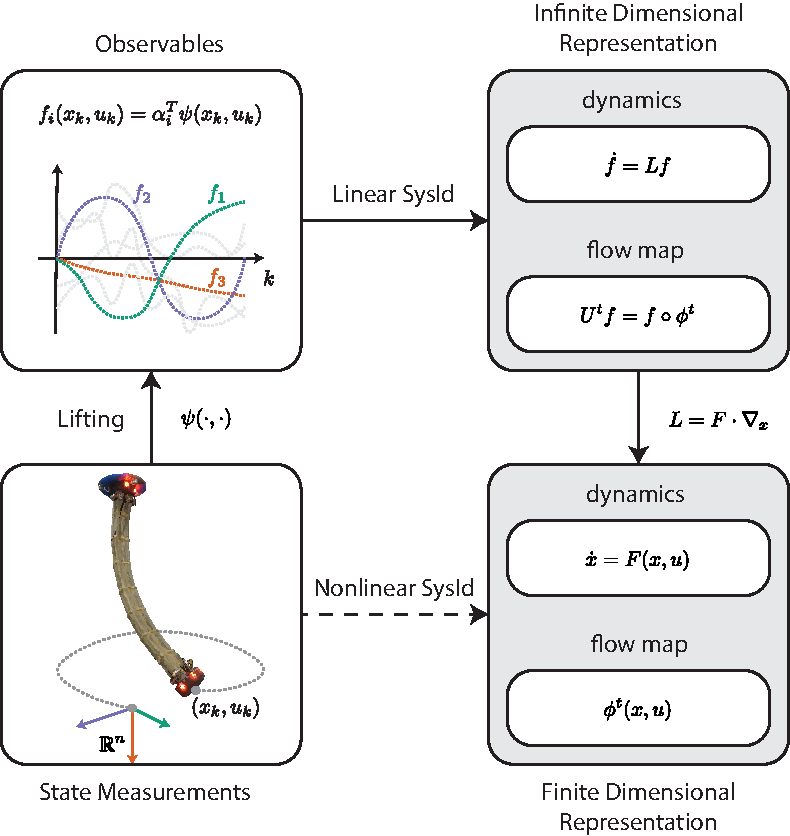
\includegraphics[width=\linewidth]{figures/overviewDiagram_v18.pdf}
    \caption{ROUGH CAPTION: 
    By providing an infinite-dimensional linear representation of a dynamical system, Koopman Operator Theory enables linear system identification of nonlinear systems. 
    This process proceeds in three steps.
    In step one, measured states of the system are lifted to the space of observables.
    In step two, least-squares regression is performed on the lifted data to obtain an approximation of the Koopman operator, $U^t$.
    In step three, the nonlinear vector field $\Fv$ is obtained via \eqref{eq:L2F} and \eqref{eq:U2L}.}
    \label{fig:overview}
\end{figure}

%% Soft robots are particularly well suited for system identification
As described earlier \David{Not a fan of the structure, as you go from `modelling is hard' to `models are important' back to `models are hard.'  I would suggest: paragraph 1: Benefits of soft robots 2: benefits of models (maybe give references of model based control) 3: types of models and examples in references (rough categorization should be along the spectrum of physics based vs. data driven) 4: challenges of physics-based models (and approximating models derived from first principles (say, linear springs, constant curvature,...)) 5: challenges of data-driven models (nonlinear vs. linear) 6: pitch for your work.}, traditional physics-based models of soft robots are typically insufficient 
% or too complex 
\Ram{complexity in terms of number of states rather than degree of the dynamics.} for control \Ram{cite a reference?}. 
As an alternative, empirical models can be built instead.
By virtue of their soft bodies it is often possible to safely command arbitrary control inputs without risk of damaging a soft robot or nearby human operators.
Thus, soft robots are amenable to data collection over their entire operation range, making them particularly well suited for data-driven system identification techniques.
% Since a white-box model based on first principles, e.g. a model for a physical process from the Newton equations, are typically unavailable or too complicated to be used in control due to the complex nature of soft robots, (grey and black box models built via) system identification are needed.
%% Linear system identification is trivial
System identification of a linear model can be performed via linear regression on observed data \cite{ljung1987system}.
However, linear models have a limited ability to capture the dynamics of soft robots which are characterized by complex nonlinear behaviors \cite{rus2015design}.
%% Nonlinear system identification is hard
Unfortunately, identifying a nonlinear model is often difficult since it consists of solving a nonlinear non-convex optimization problem, for which global convergence is not guaranteed \Ram{reference?}.

%% Neural network has successfully been applied to soft robot
Despite its challenges, nonlinear system identification of a soft robot has been performed in the past.
In \cite{gillespie2018learning}, for instance, a Deep Neural Network (DNN) was used to model the behavior of a 1 DOF pneumatic soft robot arm.
The resulting model predictive controller (MPC) with the neural network model acting as its predictor performed comparably to an MPC controller with a much more complicated physics-based model.
While in this case the neural network model was effective, a weakness of neural network models in general is the extent to which the training process is heuristic in nature.
A neural network model depends on the specific training parameters chosen (e.g. number of hidden layers, number of nodes per layer, activation function, termination condition), which must be selected through trial and error until acceptable results are achieved.
% and training may result in a sub-optimal neural network model for a given set of data.

\David{I would open here with ``In this work, we propose to employ Koopman operator theory to generate nonlinear, data driven models of soft robotic systems.'' Then add details, but but the focus on your contribution.}
%% Koopman let's us do linear sysid (trivial) on a nonlinear system
A more reliable system identification approach utilizes Koopman operator theory to perform linear system identification of nonlinear systems \Ram{what does more reliable mean?}.
This approach, which is described in greater detail in this paper \Ram{maybe say specific sections}, relies on the idea of lifting nonlinear dynamical systems to an infinite dimensional space, where those systems have a linear representation.
% \Ram{maybe these next few sentences are too much detail for now since that is something you are going to present later on...maybe just highlight its strengths? You may want to reference the figure you have developed as well.}
% \sout{The Koopman Operator is a linear operator that describes the flow of observable functions of state along trajectories of the system.
% By exploiting the lifting obtained through the Koopman operator,}
In this space, it is possible to describe the dynamic behavior of a system by identifying a linear operator in the space of observable functions instead of identifying a nonlinear vector field in the state space.
This linear operator, called the Koopman operator, is identified via linear regression, so it does not suffer from the indeterminacy of other nonlinear system identification methods.
% Since the Koopman operator is defined on an infinite-dimensional vector space, in practice it must be projected onto a finite basis of observable functions.
% However, with a suitably large finite dimensional approximation, we demonstrate that we can capture the true nonlinear system dynamics of a soft robot arm more accurately and more reliably than several other nonlinear system identification methods.

\Ram{I think you need a sentence here listing out the contributions of this paper....}
\Dan{I thought that's what this sentence does...}
\David{It's a summary of what you do.  Your contribution is more high level.  ``How do you advance the state of the art?'' vs. ``what do you do?''.  ``We propose to employ...'' vs. ``We apply...''}
In this paper we apply the Koopman based system identification method described in \cite{mauroy2016linear} and \cite{mauroy2017koopman} to create a dynamic model of a soft robot arm and demonstrate that it captures the system's true dynamic behavior better than the models generated by several other state-of-the-art nonlinear system identification methods including a neural network model, a nonlinear auto-regressive moving average model with exogenous inputs (NARMAX model), a nonlinear Hammerstein-Wiener model, and a state space model.

%% Why is this contribution significant?: Could enable real-time sysid/control, MPC, 
To the author's knowledge, this technique has never before been used to identify the dynamic model of a real system, much less a soft robot.
We believe that this system identification method applied to soft robots will enable the rapid development of new and effective control strategies by making accurate nonlinear dynamic models easier to construct.
% We believe that the models generated are accurate enough to be useful in control applications such as predictors in MPC controllers.
% Due to its numerical simplicity, this method also has the potential to be incorporated into real-time simultaneous sysid/control applications.

%% Outline of the rest of this paper
The rest of this paper is organized as follows:
In Section \ref{sec:theory} we formally introduce the Koopman Operator and describe the system identification method. 
In Section \ref{sec:experiment} we describe the soft robot and experimental procedure used for collecting input-output data of the system.
In Section \ref{sec:results} we summarize the results of applying various nonlinear system identification techniques to the collected data and compare the performances of the models generated. Concluding remarks and perspectives are provided in Section \ref{sec:conclusion}.
